\documentclass[a4paper]{article}

\usepackage[english]{babel}
\usepackage[utf8]{inputenc}
\usepackage{amsmath}
\usepackage{amsfonts}
\usepackage{graphicx}
\usepackage{minted}

\title{6.047 Computational Biology, Problem Set 1 Writeup: Aligning
and Modeling Genomes}
\author{Matthew Feng}

\date{\today}

\begin{document}
\maketitle

\section{Evolutionary distances of orthologs and paralogs}
\subsection*{a. Needleman-Wunsch}

\begin{minted}{python}
for i in range(1, len(seq1) + 1):
    for j in range(1, len(seq2) + 1):
        b1 = seq1[i - 1]
        b2 = seq2[j - 1]
        # Option 1:
        # i, j align
        opt1 = F[i - 1][j - 1] + \
               subst_matrix[base_idx[b1]][base_idx[b2]]
        # Option 2:
        # i aligns with gap, so we want to align remainder of seq1
        opt2 = F[i - 1][j] - gap_pen
        # Option 3:
        # j aligns with gap, so we want to align remainder of seq2
        opt3 = F[i][j - 1] - gap_pen
        F[i][j], TB[i][j] = max((opt1, PTR_BASE),
                                (opt2, PTR_GAP2),
                                (opt3, PTR_GAP1), key=lambda x: x[0])
\end{minted}

\noindent The code above generates the following for 
{\tt CTAAGTACT} and {\tt CATTA}:\\

{\tt
\noindent Score: -6\\
CTAAGTACT\\
C--ATTA--\\
}

\newpage
\begin{verbatim}
F(i, j) with traceback:
  0    -4    -8   -12   -16   -20
    `-.
 -4     3    -1    -5    -9   -13
        |
 -8    -1     1     2    -2    -6
        |
-12    -5     2    -1     0     1
          `-.
-16    -9    -2     0    -3     3
                `-.
-20   -13    -6    -4    -2    -1
                      `-.
-24   -17   -10    -3    -1    -4
                            `-.
-28   -21   -14    -7    -5     2
                                |
-32   -25   -18   -11    -8    -2
                                |
-36   -29   -22   -15    -8    -6
\end{verbatim}


Using the provided similarity matrix, the alignment score between
the human and mouse HoxA13 gene is $2971$.


\subsection*{b. Distance metric}
\begin{minted}{python}

F[i][j], TB[i][j] = min((opt1, PTR_BASE),
                        (opt2, PTR_GAP2),
                        (opt3, PTR_GAP1), key=lambda x: x[0])

S = [
   # A  G  C  T
    [0, 1, 2, 2], # A
    [1, 0, 2, 2], # G
    [2, 2, 0, 1], # C
    [2, 2, 1, 0]  # T
]

gap_pen = -4 # add penalty instead of subtract
\end{minted}

In order to convert the standard similarity matrix into a matrix
that would generate alignment scores that could be used as distances,
I had to change two things in the alignment program:
\begin{enumerate}
\item First, if two symbols match, then they should have a distance of 0;
Furthermore, the more dissimilar two symbols are, the greater (instead
of smaller) the value they should have in matrix $S$. Additionally, since
we subtract the gap penalty, the gap penalty must now be negative
instead of positive. To achieve all these changes, I changed the values
along the main diagonal of $S$ to $0$, and flipped the signs of all
other values.
\item Second, because we are now dealing with finding the minimum distance
instead of the maximum score, I had to change the aggregating function
in the dynamic programming loop from {\tt max} to {\tt min}.
\end{enumerate}

\subsection*{c. Distance between human and mouse HoxA13}
Using the modified ``similarity'' (since now we are in effect
measuring differences) matrix $S$ defined in part (b), the
distance between the human and mouse HoxA13 gene is $197$.

\subsection*{d. Dating HoxA13 and HoxD13}
Again, using the modified ``similarity'' matrix $S$ defined in part (b),
the distance between the human HoxA13 and human HoxD13 gene is $1145$,
and the distance between the mouse HoxA13 and mouse HoxD13 gene is $1095$.

If we assume that the alignment score can be used as a distance metric,
that the distance metric is consistent across mutations and species,
and that it is linear in that $c \times \text{dist}(a, b)$ implies that
the evolutionary age between $a$ and $b$ is $c$ times older, then
we can estimate the date that whole-genome duplication gave rise to HoxA13
and HoxD13. Concretely, since $197$ corresponds to a date $70$ million
years ago, then $\frac{1145}{197} \times 70 = 290.6$ million years ago
for the divergence of human HoxA13 and HoxD13, and
$\frac{1095}{197} \times 70 = 277.9$ million years ago for
mouse HoxA13 and HoxD13 divergence.

\section{Sequence hashing and dotplot visualization}

\subsection*{a. Exact 30-mers}

\begin{verbatim}
$ python ps1-dotplot.py human-hoxa-region.fa \
> mouse-hoxa-region.fa human-mouse-hoxa-30-mer.png
62829 hits found
24.70197% hits on diagonal
\end{verbatim}

The off diagonal hits formed a grid like shape in the
graph, which means that hits were found in a steady,
repeated pattern. These hits that were not along the 
diagonal could possibly be promoter sequences and oriC
locations, which appear repeatedly in a DNA sequence.

Matches along the diagonal are more likely to be ``correct'',
or orthologous alignments because we reason that the two
sequences we want to align are reasonably related, and so
differences between the two should not span a large distance,
i.e. pieces that were related previously should still be
in close proximity to their origin, and if both sequences
come from the same origin, the hits should be near the same place,
which appears as ``along the diagonal'' in our graph.

\subsection*{b. Variations}
\subsubsection*{i. Exact 100-mers}
\begin{verbatim}
$ python ps1-dotplot.py human-hoxa-region.fa \
> mouse-hoxa-region.fa human-mouse-hoxa-100-mer.png
1198 hits found
100.00000% hits on diagonal
\end{verbatim}
Many fewer hits were found, so the graph looked
particularly sparse, but all the hits that were found
were along the diagonal.

\subsubsection*{ii. 60-mers}
\begin{verbatim}
$ python ps1-dotplot.py human-hoxa-region.fa \
> mouse-hoxa-region.fa human-mouse-hoxa-60-mer.png
23933 hits found
38.74149% hits on diagonal
\end{verbatim}
Accordingly, 60-mers had more hits than 100-mers and
fewer hits than exact 30-mers because of the increased
length, but had many more than the 100-mers because of
the flexibility of only every other symbol needing to
match.

\subsubsection*{iii. 90-mers}
\begin{verbatim}
$ python ps1-dotplot.py human-hoxa-region.fa \
> mouse-hoxa-region.fa human-mouse-hoxa-90-mer.png
8887 hits found
93.85619% hits on diagonal
\end{verbatim}
As a length of 90 is large, the number of hits decreased
correspondingly; however, we had many more hits than the
exact 100-mer again because of the requirement that only
every third base match, rather than every base.

\subsubsection*{iv. 120-mers}
\begin{verbatim}
$ python ps1-dotplot.py human-hoxa-region.fa \
> mouse-hoxa-region.fa human-mouse-hoxa-120-mer.png
6044 hits found
82.13104% hits on diagonal
\end{verbatim}
The number of hits decreased once again, and the specificity
decreased as well, since we were checking too few bases along
the entire k-mer.

\subsubsection*{v. 100-mers with mismatches}
In order to implement this, I would first hash every sixth
base in a length of 100 monomers, and find the hits 
based on the simple every sixth base heuristic. Afterwards,
however, I would filter each hit in linear time to determine
if the hit satisfies the constraint that only two mismatch
for every contiguous block of six. Checking for this
additional constraint takes ~$100$ operations per hit,
and with fewer than $10,000,000$ hits, this is computationally
feasible on a modern computer.

\subsection*{c. Specificity to the diagonal}
Having the 90-mer that matched every third base was the most
specific to the diagonal, having $93.86\%$ of the hits be
located along the diagonal. This is likely due to the right
balance of the length of the k-mer we are trying to hit and
the spacing between each monomer we actually check for
equivalence. For a 120-mer, there were many more options in
between the 30 bases that we checked to match, and so fewer
were specific to the diagonal. With the 60-mers, we
still only checked quite a short length of sequence for
alignment, which allowed for many more substrings to match,
which also resulted in a lower specificity.

\subsection*{d. Sensitivity vs. Specificity}
If the length of the k-mer we are hashing is low, then we
get many more hits (sensitivity increases), but a fewer
percentage of those fall along the diagonal, because we
are too lenient with our matching. Likewise, if the length
of the k-mer is too long, then most matches we have are along
the diagonal, but we have much fewer matches (specificity
is much higher). Hashing only every $n$th symbol in a sequence
allows us to match more hits; the larger $n$ is, the more
hits we are likely to find (because we allow for many more
single symbol mismatches). In other words, increasing $n$
trades specificity for sensitivity.

\subsection*{e. Inversions}
The inversion ranges from indices {\tt [54549, 290751)}. The
inversion can be found by checking the reverse of every 200-mer
against the original order 200-mer hashes, and look for a
large section of matches. We can then look at the list of
hits and find the first in the large chunk, and find the last
as well.

\begin{minted}{python}
# to find the last in the large chunk of hits
for i in xrange(len(seq2) - 1, -1, -1):
    key = seq2[i:i + kmerlen]
    key = key[::kmerskip]
    key = invert(key)

    # store hits to hits list
    any_hits = lookup.get(key, [])
    if len(any_hits) != 0:
        chain.append(i)
        if len(chain) > 50:
            print(max(chain))
            quit()
    else:
        chain = []

# to find the first in the large chunk of hits
for i in xrange(0, len(seq2) - kmerlen + 1):
    key = seq2[i:i + kmerlen]
    key = key[::kmerskip]
    key = invert(key)

    # store hits to hits list
    any_hits = lookup.get(key, [])
    if len(any_hits) != 0:
        chain.append(i)
        if len(chain) > 50:
            print(min(chain))
            quit()
    else:
        chain = []
\end{minted}

\begin{figure}
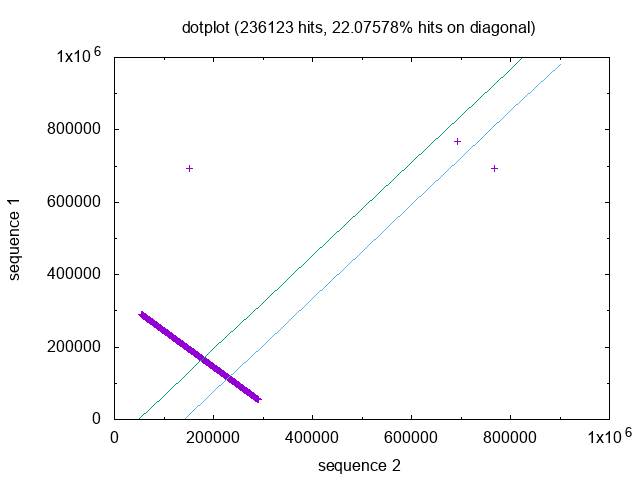
\includegraphics[width=\textwidth]{./human-hoxa-inverted.png}
\end{figure}

\section{HMMs for GC-rich regions: State durations and limitations}

\subsection*{a. State durations}
Let $D_k$ represent the duration of staying in state $k$. Then the
distribution of state durations $D_k$ is a random variable that follows a
{\bf geometric distribution}, defined as the number of failures
before the first success, if we consider a {\it success} as transitioning out of 
state $k$.

More concretely, the probability distribution function of $D_k$ is
\[
p_{D_k}(d) = \mathbb{P}(D_k = d) = (1 - p)^{d - 1}p
\]
where $p$ is the probability of transitioning out of state $k$ (i.e. from state $k$
to another state $k' \neq k$). The expected value of state duration
$D_k$ is
\[
    \mathbb{E}[D_k] = \frac{1}{p} - 1
\]
where again, $p$ is the probability of transitioning out of state $k$.

\subsection*{b. Viterbi algorithm}
Based on the transition probabilities hardcoded into the program, 
the expected duration for both high and low GC regions 
should be $99$ (since we don't count the transitioning out state).

\subsection*{c. Mystery sequences}
\subsubsection*{Mystery 1}
{\tt
Authoritative annotation statistics\\
-----------------------------------\\
High-GC mean region length:  100\\
High-GC base composition: A=19.94\% G=29.87\% C=30.20\% T=20.00\%\\
Low-GC mean region length:  101\\
Low-GC base composition: A=29.87\% G=20.27\% C=19.73\% T=30.13\%\\

\noindent Viterbi annotation statistics\\
-----------------------------\\
High-GC mean region length:  234\\
High-GC base composition: A=20.51\% G=29.18\% C=29.40\% T=20.91\%\\
Low-GC mean region length:  220\\
Low-GC base composition: A=29.62\% G=20.66\% C=20.20\% T=29.52\%\\

\noindent >> Accuracy: 71.96\%\\
}

In mystery 1, the distribution of authoritative state
durations was more or less uniform from lengths of $40$
to $140$ for both high and low GC content. However, the Viterbi
decoding found regions with duration ranging from $50$ to $900$,
with a mode around $100$ and a long right tail.

\subsubsection*{Mystery 2}
{\tt
Authoritative annotation statistics\\
-----------------------------------\\
High-GC mean region length:  100\\
High-GC base composition: A=19.85\% G=29.78\% C=30.07\% T=20.30\%\\
Low-GC mean region length:  99\\
Low-GC base composition: A=29.84\% G=19.86\% C=19.99\% T=30.31\%\\

\noindent Viterbi annotation statistics\\
-----------------------------\\
High-GC mean region length:  214\\
High-GC base composition: A=20.56\% G=29.15\% C=29.46\% T=20.83\%\\
Low-GC mean region length:  212\\
Low-GC base composition: A=29.16\% G=20.45\% C=20.56\% T=29.83\%\\

\noindent >> Accuracy: 68.80\%\\
}

In mystery 2, the distribution of authoritative state
durations for high GC content was normally distributed with 
mean of $100$ and standard deviation of $9.75$; for low GC content,
the distribution was normal with mean $99$ and standard deviation
of $10.7$. Again, however, the Viterbi decoding found regions
with lengths ranging from $50$ to $1000$, with a mode around $100$
but a very long right tail. In other words, the Viterbi decoding
found a geometric-like distribution for the state durations, rather
than the true, normal distribution.

\subsubsection*{Mystery 3}
{\tt
Authoritative annotation statistics\\
-----------------------------------\\
High-GC mean region length:  100\\
High-GC base composition: A=19.81\% G=29.71\% C=30.56\% T=19.91\%\\
Low-GC mean region length:  100\\
Low-GC base composition: A=29.56\% G=20.09\% C=20.11\% T=30.24\%\\

\noindent Viterbi annotation statistics\\
-----------------------------\\
High-GC mean region length:  221\\
High-GC base composition: A=20.56\% G=29.05\% C=29.84\% T=20.55\%\\
Low-GC mean region length:  207\\
Low-GC base composition: A=29.10\% G=20.46\% C=20.53\% T=29.91\%\\

\noindent >> Accuracy: 67.72\%\\
}

In mystery 3, the distribution of authoritative state durations was
a constant length of $100$ for both high and low GC content. However,
the Viterbi decoding, using the provided parameters, still found
region durations in the bimodally around durations of $80$ and $230$
with a long right tail, causing the mean to be skewed to $221$ and $207$
for high and low GC regions, respectively. Because the state durations
were not accurately modeled by the topology and parameters of the HMM,
the HMM only achieved an accuracy of $67.72\%$.

In all three of the mystery sequences, the authoritative
state durations for both high and low GC content never
exceeded $200$; however, the Viterbi decoding consistently
determined sequences with durations greater than $200$.

\subsection*{d. Retraining the HMM parameters}
Even if we had correctly annotated sequences for the
mystery sequences, I do not believe that performance
of the Viterbi algorithm, using the supervised learning
training procedure discussed in class, would improve.
The reason is that all the authoritative sequences
had a mean duration of around 100; to get the MLE for
this mean duration, the transition probabilities $a_{kl}$
would be assigned the same (or very similar) values to
they are now, because the expected value of the transition
probability is the mean value of the actual durations.
The problem steps from our topological assumption that
durations depend only on the single previous state, which
leads to an assumed geometric or exponential distribution,
rather than the true distribution.

\subsection*{e. GENSCAN}
GENSCAN overcomes the inherent assumption of Markov Chains
that duration distributions are geometric by {\it allowing
the probability of transition to depend on the amount
of time that the model has been in a certain state}; in
other words, GENSCAN takes advantage of a semi-Markov property,
also known as a hidden semi-Markov model. Hidden semi-Markov
models allow for any state duration distribution to be modeled,
rather than be confined to geometric distributions. We can
implement HSMMs by defining transition and emission probabilities
as functions of time rather than constants, and keep a 
record of the current duration when computing the parameters.

\section{Final project preparation}

The responses to this question are in {\tt FengMatthew\_Profile.docx}.

\end{document}